\documentclass[10pt]{JoME}

\usepackage{hyperref}
\usepackage{graphicx}

% to be set by Editor:
% ------------------------------------------------------------------------------------------------------------------
%\renewcommand{\svCorr}{*Corr. Author's Address: Name of institution, Address, City, Country, \email{xxx.yyy@wwww.zzz}}
\renewcommand{\svSV}{Strojniški vestnik - Journal of Mechanical Engineering 63(2017)3,  XXX-4}
%\renewcommand{\svAuthors}{Author-A, Author-B}
\renewcommand{\svCyear}{2017}
\renewcommand{\svDOI}{DOI: 10.5545/sv-jme.2017.4027}
\svDates{2016-11-04}{2017-01-14}{2017-02-12}
\renewcommand{\svType}{Review Paper}
% ------------------------------------------------------------------------------------------------------------------

\svTitle{Title of the paper}
\author{
Author's Name Surname\svMark{1,*}  - Co-author's Name Surname\svMark{2} \\
\svAffil{1}{Author's institution} \\
\svAffil{2}{Co-Author's institution}
}
%\date{\today\  -- \clock}
\date{}

\crop[cross,axes]
%\crop[frame,axes]
%\crop[off]

\begin{document}
\twocolumn[\begin{svHead}

\begin{svAbstract}
The Abstract should not exceed 250 words. The Abstract should state the principal objectives and the scope of the investigation, as well as the methodology employed. It should summarize the results and state the principal conclusions. An effective abstract stands on its own — it can be understood fully even when made available without the full paper. To this end, avoid referring to figures or the bibliography in the abstract. Please introduce any acronyms the first time you use them in the abstract (if needed), and do so again in the full paper. About 4 to 6 significant key words should follow the abstract to aid indexing.
\end{svAbstract}

\svKeywords{key word, key word, key word, key word, key word}

\begin{svHigh}
\item Highlights (4 to 6) are a short collection of bullet points that convey the core findings and provide readers with a quick textual overview of the article. 
\item These four to six bullet points should describe the essence of the research (e.g. results or conclusions) and highlight what is distinctive about it. 
\item See latest SV-JME papers for examples.
\end{svHigh}

\end{svHead}]

 
\section{INTRODUCTION}

An Introduction should provide a review of the recent literature on the topic and sufficient background information to allow the results of the article to be understood and evaluated. 

In the Introduction section, state the motivation for the work presented in your paper and prepare readers for the structure of the paper. Write four components, preferably (but not necessarily) in four paragraphs: \emph{context}, \emph{need}, \emph{task}, and \emph{objective} of the article.

First, provide some \emph{context} to orient those readers who are less familiar with your topic and to establish the importance of your work.

Second, state the \emph{need} for your work, as a comparison between what the scientific community currently has and what it wants.

Third, indicate what you have done in an effort to address the need (this is the \emph{task}).

Finally, preview the remainder of the paper to mentally prepare readers for its structure, in the \emph{objective} of the document.

Please note that heading numeration for this chapter starts with 0.
%\vfill

\section{METHODS}

The Methods section details the theoretical or experimental methods used. What justifies using a given method? What is special, unexpected, or different in your approach? If you use a standard or usual procedure, mention that upfront, too.


\section{EXPERIMENTAL}

The Experimental section should provide details of the experimental set-up and the methods used to obtain the results. To make this section interesting, explain the choices you made in your experimental procedure. This section should provide sufficient detail for other scientists to be able to reproduce the experiments presented in this paper.

The Methods and Experimental part may be combined. 

\begin{figure*}
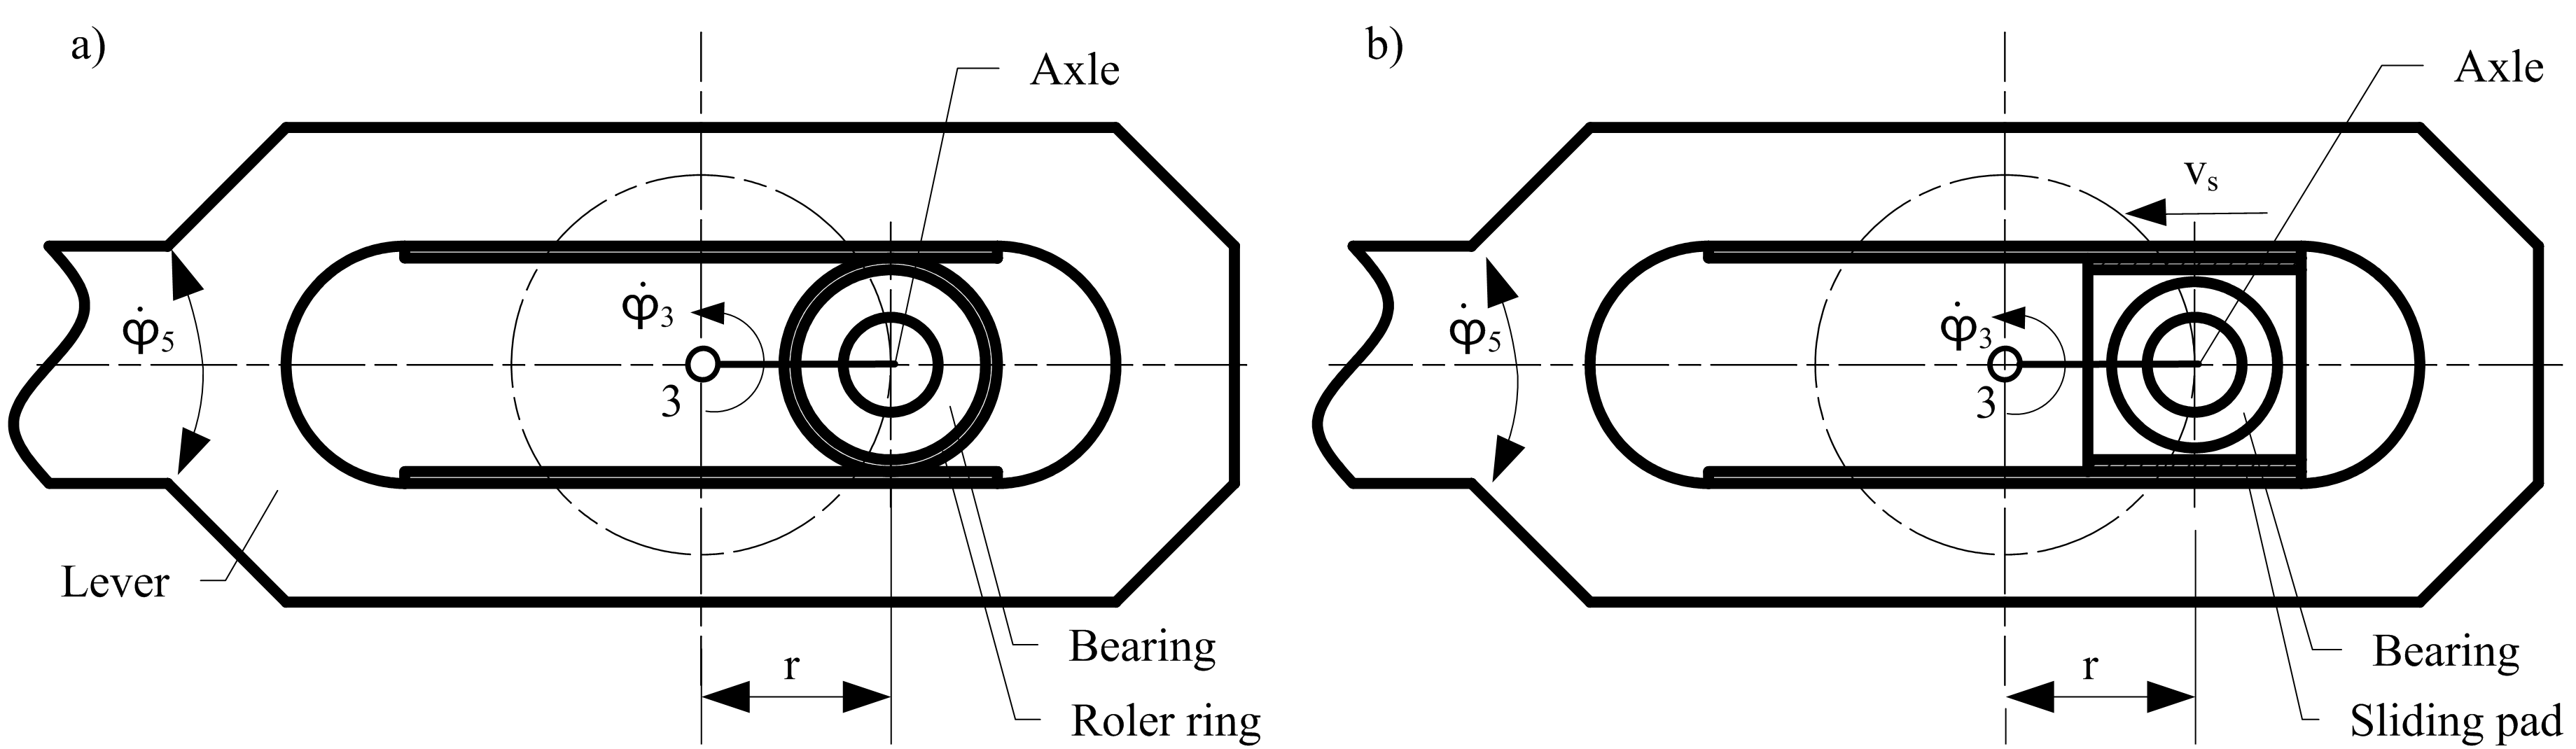
\includegraphics[width=161mm]{fig1.png}
\caption{A figure title; a) explanation of part a; and b) explanation of part b\label{figA}}
\end{figure*}

\subsection{Subtitle 1}
You may organize the body of your paper into subsections or sub-subsections; however, remember to prepare your readers for the structure ahead at all levels.

\subsection{Special Notes}
You can similarly prepare your readers for an upcoming division into subsections by introducing a global paragraph between the heading of a section and the heading of its first subsection. This paragraph can contain any information relating to the section as whole rather than particular subsections, but it should at least announce the subsections, whether explicitly or implicitly.


\subsubsection{Article Types}
\emph{Original scientific paper} (1.01): Scientific papers should report significant and innovative results and exhibit a high level of originality. \emph{Review scientific papers} (1.02): Review articles are in the form of systematic reviews and literature reviews and are a form of secondary literature. Systematic reviews determine an objective list of criteria and find all previously published original experimental papers that meet the criteria. They then compare the results presented in these papers with proposed innovative or novel findings. \emph{Short scientific papers} (1.03): These generally have the same structure as longer scientific papers but are shorter (max 6 pages) and report on a significant, but limited, aspect of research work meriting a separate publication.

\subsubsection{Units}
The SI system of units for nomenclature, symbols and abbreviations should be followed closely. Symbols for physical quantities in the text should be written in italics (e.g. $v$, $T$, $n$, etc.). Vectors and matrix should be written in bold. See Eq. (2). Symbols for units that consist of letters should be in plain text (e.g. ms$^{-1}$, K, min, mm, etc.). 

Please also see:\\ \href{http://physics.nist.gov/cuu/pdf/sp811.pdf}{http://physics.nist.gov/cuu/pdf/sp811.pdf}.

\subsubsection{Abbreviations}
Abbreviations should be spelt out in full on first appearance followed by the abbreviation in parentheses, e.g. variable time geometry (VTG). The meaning of symbols and units belonging to symbols should be explained in each case or cited in a nomenclature section at the end of the manuscript before the References.

\subsubsection{Figures}
Figures (figures, graphs, illustrations digital images, photographs) must be cited in consecutive numerical order in the text and referred to in both the text and the captions as Fig.~\ref{figA}, Fig.~\ref{figB}, etc. Figures should be prepared without borders and on white grounding and should be sent separately in their original formats. If a figure is composed of several parts, please mark each part with a), b), c), etc. and provide an explanation for each part in Figure caption. The caption should be self-explanatory. Letters and numbers should be readable (Arial or Times New Roman, minimum 6 pt, with equal sizes and fonts in all figures).

\begin{figure}[h]
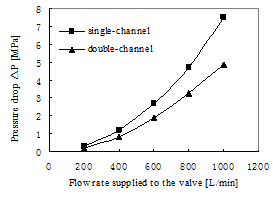
\includegraphics[width=76.5mm]{fig2.png}
\caption{Pressure drops in the DN25 valve using different structures\label{figB}}
\end{figure}
 
 
\textbf{Graphics} (submitted as supplementary files) may be exported in resolution good enough for printing (min. 300 dpi) in any common format, e.g. TIFF, BMP, GIF or JPG, PDF, zipped in one or more files, and uploaded as supplementary files. However, graphs and line drawings should be prepared as vector images, e.g. CDR, AI. Do not upload figures in word format.
Multi-curve graphs should have individual curves marked with a symbol or otherwise provide distinguishing differences using, for example, different thicknesses or dashing. Please see Figs.~\ref{figB} and \ref{figC}.

  
\begin{figure}[h]
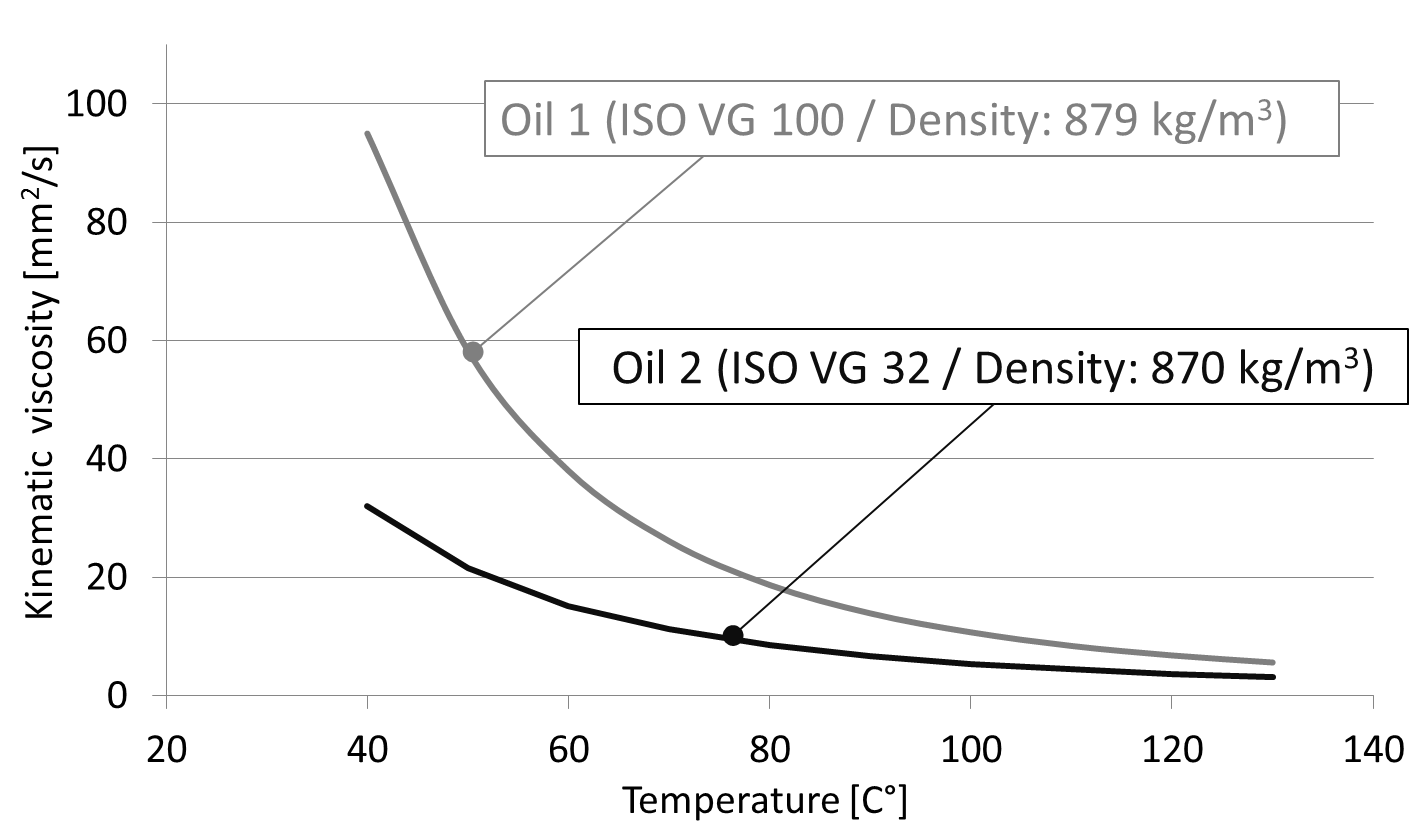
\includegraphics[width=76.5mm]{fig3.png}
\caption{Effect of temperature on the viscosity of the test oils\label{figC}}
\end{figure}
 
  

Please omit simulation print screens. Where they are irreplaceable the figures should be prepared at a professional designer’s level, ready to be printed, but not as shown in Fig.~\ref{figD}. In this figure there are several issues to be avoided such as: incomplete text, unreadable texts and legend, missing units in the legend, contrast issue, etc. When converting a figure to a Black \& White printing technique a reader cannot tell what darker shades (red and blue) represent. Are they a maximal or minimal values? 

\begin{figure}[h]
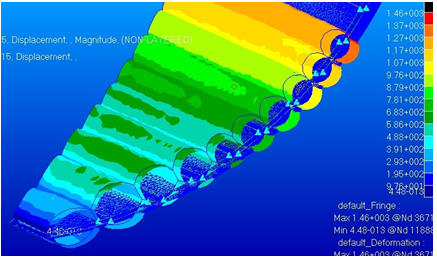
\includegraphics[width=76.5mm]{fig4.png}
\caption{A simulation print screen using a colour technique\label{figD}}
\end{figure}


\subsubsection{Tables}

Tables should carry separate titles and must be numbered in consecutive numerical order in the text and referred to in both the text and the captions as Table 1, Table 2, etc. Tables should not duplicate data found elsewhere in the manuscript. Tables should be prepared using a table editor and not inserted as a graphic.

\begin{table}[h]
\caption{Table title\label{tabA}}
\medskip\fontsize{10}{12}\selectfont
\begin{tabular}{lccc}
\hline
LDF	& Line &	Point  & Precision \\
          &  defects &  defects  &  [\%] \\
\hline
Real quantity  & 86   &  214  &   \\
Number of true positives  & 65	& 213 &  92.7  \\   	
Number of false positives & 21 & 1	\\
\hline
\end{tabular}
\end{table}

\subsubsection{Equations}

Equations should be numbered in consecutive numerical order with the use of brackets in the text and referred in the text as Eq. (1), Eq. (2), etc. The equation editor should be used for composing equations. In addition to the physical quantities, variables such as t should be in italics, matrixes, vectors and tensors, such as one in Eq.~(\ref{eqB}) in bold, the constants in normal text (c1) and the units (normal text) should be added in square brackets. See Table~\ref{tabA}.

\begin{equation}\label{eqA}
f(x) = \mbox{arg}\max_{y \in Y} F(x,y),
\end{equation}

\begin{equation}\label{eqB}
\mathbf{T} = \left[\begin{array}{ccc} 1 & 0 & -367 \\  0 & 1 & 0 \\ 0 & 0 & 1 \end{array}\right] .
\end{equation}


\subsubsection{Decimal Notation}

A period/full stop (never a comma) is used as the decimal point (6.57, not 6,57). The number of decimal places should be consistent within a list or context (The response rates were 41.0 and 47.4 percent, respectively, not 41 and 47.4 percent), unless different precisions are actually intended. Nouns following a number expressed as a decimal are plural (averaging 0.7 years).



\section{RESULTS}

The Results section should clearly and concisely present the data, using figures and tables where appropriate. State the message of each paragraph upfront: Convey in the first sentence what you want readers to remember from the paragraph as a whole. Focus on what happened. Then develop your message in the remainder of the paragraph, including only that information (figures and tables) you think you need to convince your audience.

\section{DISCUSSION}

The Discussion section that should describe the relationships and generalizations shown by the results and discuss the significance of the results, making comparisons with previously published work. It may be appropriate to combine the Results and Discussion sections into a single section to improve clarity.

\section{CONCLUSIONS}

A Conclusions section should present one or more conclusions drawn from the results and subsequent discussion. It should state the most important outcome of your work. This should not duplicate the Abstract. You may also consider including perspectives -- that is, an idea of what could or should still be done in relation to the issue addressed in the paper.

\section{ACKNOWLEDGEMENTS}

Acknowledgement (optional) of collaboration or preparation assistance may be included. Please note the source of funding for the research.

\section{NOMENCLATURES}

Nomenclature (optional). Papers with many symbols should include a nomenclature that defines all symbols with units, inserted above the references. If one is used, it must contain all the symbols used in the manuscript and the definitions should not be repeated in the text. In all cases, identify the symbols used if they are not widely recognized in the profession. Define acronyms in the text, not in the nomenclature.\smallskip\\ 
\begin{tabular}{lll}
$v_i$	& [ms$^{-1}$] & velocity in ith position\\
$t_{max}$	& [min]  & maximal time limit\\
$T_0$	& [K]	& initial temperature
\end{tabular}

\section{REFERENCES}

A reference list must be included using the following information as a guide. Only cited text references are to be included. All references must be complete and accurate. Please add DOI code when available. Examples follow.
 
\textrm{\textbf{Journal Papers}  \cite{bib1}: 
Surname 1, Initials, Surname 2, Initials (year). Title. \textit{Journal}, volume, number, pages, DOI code. Journal titles should not be abbreviated. Note that \textit{Journal Title} is set in italics.} 

\textrm{\textbf{Books} \cite{bib2}: Surname 1, Initials, Surname 2, Initials (year). \textit{Title}. Publisher, place of publication. Note that the \textit{Title of the Book} is italicized.} 

\textrm{\textbf{Chapters in Books} \cite{bib3}:
Surname 1, Initials, Surname 2, Initials (year). Chapter title. Editor Surname 1, Initials, Editor Surname 2, Initials (ed(s).), \textit{Book title}. Publisher, place of publication, pages. Note that the \textit{Book title} is italicized.}

\textrm{\textbf{Proceedings Papers}  \cite{bib4}:
Surname 1, Initials, Surname 2, Initials (year). Paper title. \textit{Proceedings title}, pages. Note that the \textit{Proceedings Title} is italicized.}

\textrm{\textbf{Standards} \cite{bib5}: Standard-Code (year). \textit{Title}. Organisation. Place. Note that the \textit{Title of the Standard} is italicized.}

\textrm{\textbf{WWW pages} \cite{bib6}: 
Surname, Initials or Company name. Title, from \textit{http://address}, date of access. Note that the \textit{www address} is italicized.}
 
\bibliographystyle{phcpc}

\bibliography{biblio}{}

%\newpage
\section{APPENDIX}

Appendix(-ices) if any. In some cases detailed information for other scientists is placed in the appendix, primarily because it is not what most readers want to know first.

 
\end{document}

% =========================================================================

	
	

